%----------------------------------------------------------------------------------------
%	PART
%----------------------------------------------------------------------------------------

\part{Processor Design}

%----------------------------------------------------------------------------------------
%	CHAPTER 3
%----------------------------------------------------------------------------------------

\chapterimage{chapter_head_1} % Chapter heading image

\chapter{Presenting Information}

Machine oriented languages are more commonly known as assembly language. They are typically structured as one to one mappings to processor op codes (as we have seen earlier). However, assembly languages  also involve constructs (like psuedo instructions), macros and labels, all of which aid the programmers in writing programs and are not typically a one to one mapping to op codes.

\chapter{Microprogram Sequencer}

\section{Introduction}

We will start by defining a few terms

\begin{enumerate}
\item \textbf{Control Signal} It refers to the signal sent to a component (Register,ALU) to do a specific job. Also known as a Micro-operation. Example -
    \begin{enumerate}
    \item \textit{EPC} - Enable Program Counter To Bus,
    \item \textit{LOR} - Load Operand Register From Databus.
    \end{enumerate}
\item \textbf{Micro-instruction} The control signals are combined into control words, where each bit of the control word represents a signal. A control word is a micro-instruction. Example -
    \begin{enumerate}
    \item \textit{ EAR } \textit{LMR} ---- [MR] = [AR]
    \end{enumerate}
\item \textbf{Micro-program} A sequence of micro-instructions that are normally characterised by an assembly mnemonic i.e. an instruction.
\end{enumerate}

Now, A micro-program sequencer works in a way to generate these control signals from the microprogram by transitioning from one state to another in every clock cycle. A state is defined by the micro-instruction that has to be run in that clock cycle.It has two main functions 

\begin{enumerate}
    \item \textbf{Control Function} The micro-operations that need to be executed to perform a certain micro-instruction are to be defined and be known. The micro-operation(s) are dependent on parameters like selected destination, operand etc.
    \item \textbf{Sequencing Function} The address of next micro-instruction to be executed is generated while controlling test conditions etc.
\end{enumerate}

Thus, to summarize, to execute an instruction, the microprogram sequencer executes a micro-instruction in every clock cycle and determines which micro-instruction (state) to run next. It can be thought in terms of a state diagram.

\section{Work Flow}

\begin{figure}[h]
    \begin{center}
        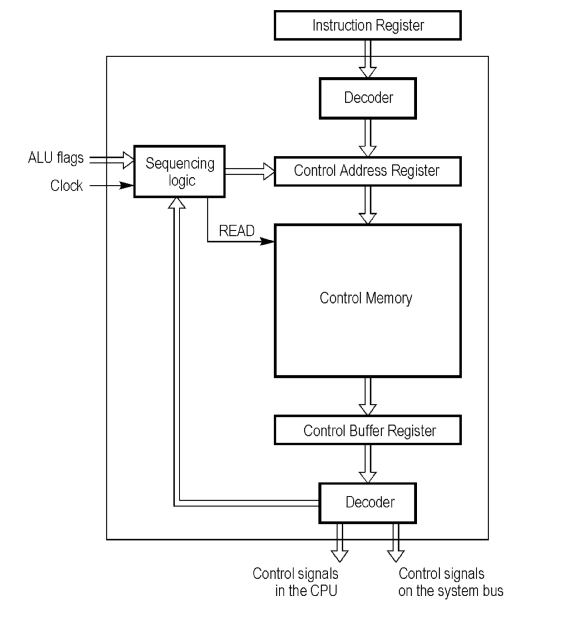
\includegraphics[scale=0.3]{MicroSequencer}
    \end{center}
    \caption{Flow of the Control Unit}
\end{figure}

The Instruction Register loads the opcode into the decoder which then translates the opcode into a control memory address. The control address register contains the address of the next micro-instruction to be read.

The micro-instructions are stored in the microprogram memory (also called control memory, can be used interchangeably). The address from the control address register is used to read from this microprogram memory.


When a micro-instruction is read from the microprogram memory, it is transferred to the control buffer register. This register activates the control signals.

\begin{figure}[h]
    \begin{center}
        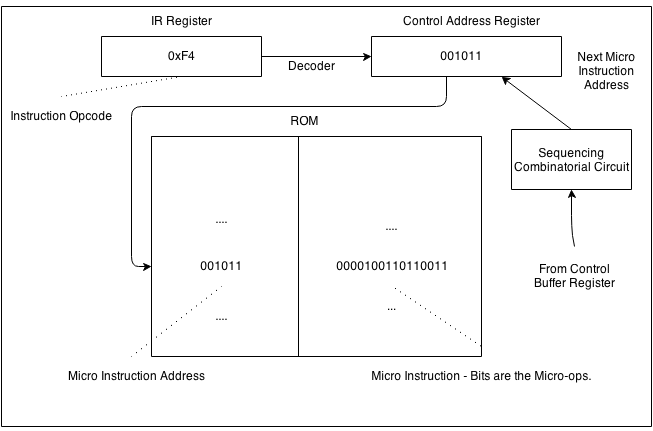
\includegraphics[scale=0.45]{SequencerTables}
    \end{center}
    \caption{The various addresses referred can get confusing.}
\end{figure}

\textit{I know you can see another decoder between the 
Control Buffer Register before the signals are sent. We will talk about this later.}
    
Thus, reading a micro-instruction from the microprogram 
memory has the effect of executing that micro-instruction.

The sequencing logic loads the control address register and 
activates the read signal. This read signal loads the next micro-instruction from the Instruction Register completing a cycle.

\section{Writable Control Memory}

Rather than storing the micro instructions in the ROM, if we would use Flash Memory or RAM, then the design has a Writable Control Memory. This has benefits including the ease of patching the microprogram and, for certain hardware generations, faster access than ROMs could provide. User-programmable Writable Control Memory allows the user to optimize the machine for specific purposes.

\section{Breadth in Microprogram Sequencer Designs}

\subsection{Horizontal and Vertical Programming}

We noticed that there was another decoder in Figure 1, this is the characteristic of a type of microcode architecture called Vertical Programming. The other variant Horizontal Programming, does not have the decoder circuit.

In horizontal microcode architecture, each control signal is represented by a bit in the micro instruction, while in the vertical microcode architecture, a set of true signals is represented in the micro instruction in a shorter form. Thus the decoder is used to convert this shorter code into true signals.

Practically, a diagonal architecture is used, combining both horizontal and vertical programming designs.

\subsection{Hardwired vs Micro-Programmed Control Units}

Hardwired control units are implemented through use of sequential logic units, using finite number of gates to generate specific results based on the last and the cuurent instruction, similar to what we have seen earlier in synchronous circuit design. Their design uses a fixed architecture—it requires changes in the wiring if the instruction set is modified or changed. Hardwired control units are generally faster than micro-programmed designs. However they are difficult to design as the instruction set starts to grow bigger. 

Microcode simplified the job by allowing the assembly instructions to be defined via microprograms rather than by circuitry. Even late in the design process, microprogram for an instruction could easily be changed, whereas hard-wired CPU designs were very cumbersome to change. Thus, this greatly facilitated CPU design.

\clearpage

\section{Example - Using IIIT Processor Instruction Set Architecture}

We will be taking an taking up an example code and stage by stage break it down into its components to understand the sequence.

Let us take the following
\begin{verbatim}    
movi r0
01
movs r0
\end{verbatim}
\textit{movi} corresponds to the 0x9* opcode family, thus \textit{movi r0} is 0x90 \\
\textit{movs} corresponds to the 0x7* opcode family, thus \textit{movs r0} is 0x70


These instructions can be broken down into, each of which will act as a state of the Microprogram Sequencer
\begin{enumerate}
\item 0x90 \textit{(movi r0)}
    \begin{enumerate}
    \item \textit{EPC, LMR, IPC}
    \item \textit{RD, LMS, LIO, LIR}
    \item \textit{EPC, LMR, IPC}
    \item \textit{RD, LRG, RMS; SRG = 0} 
    \end{enumerate}
\item 0x70 \textit{(movs r0)}
    \begin{enumerate}
    \item \textit{EPC, LMR, IPC}
    \item \textit{RD, LMS, LIO, LIR}
    \item \textit{ERG, LAR, RMS; SRG = PASSO}
    \end{enumerate}
\end{enumerate}

\textbf{\textit{The SRG is generated from opcode by the I/O register, and thus is not needed to be present in the Microprogram Memory.( We'll call it ROM after this)}}

The first two states are fetch in both the instructions and thus we assume here that they have been executed and now the next instruction, 1.(c) is going to be executed.

\begin{figure}[h]
    \begin{center}
        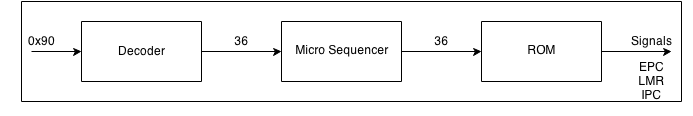
\includegraphics[scale=0.6]{InitFlow}
    \end{center}
    \caption{Flow of instruction 1.(c)}
\end{figure}

The states are stored in the ROM have a design dependent address. Let it contain state 2.(c) at address 34, 1.(c) at address 36 and state 1.(d) at address 37. The decoder has the said mapping of the states. The translated opcode ie, the address is fed to the Control Address Register which passes it to the ROM which then generates the signals. 

\begin{figure}[h]
    \begin{center}
        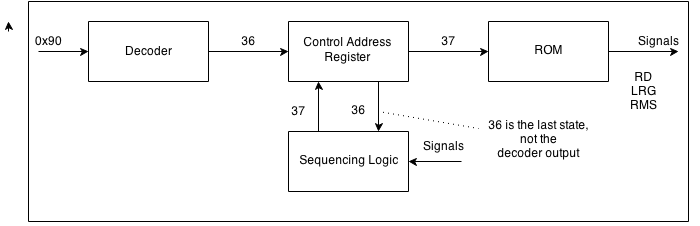
\includegraphics[scale=0.6]{SecondFlow}
    \end{center}
    \caption{Flow of instruction 1.(d)}
\end{figure}

\textbf{Also, the sequencing logic is then activated to change the address present in the Control Address Register to the next state.} The sequencer has thus jumped to the next state 1.(d).

The RMS control that is seen in this micro-instruction clear the Micro Sequencer to the reset value (ie. the initial state), usually zero.

\begin{figure}[h]
    \begin{center}
        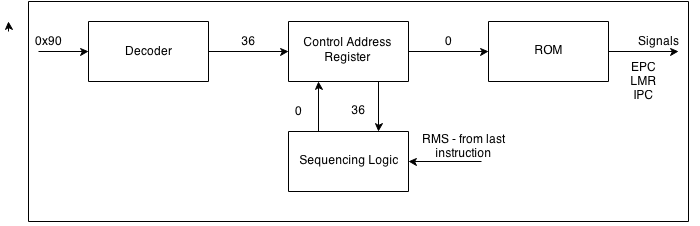
\includegraphics[scale=0.6]{FourthFlow}
    \end{center}
    \caption{Flow of instruction 2.(a)}
\end{figure}


\begin{figure}[h]
    \begin{center}
        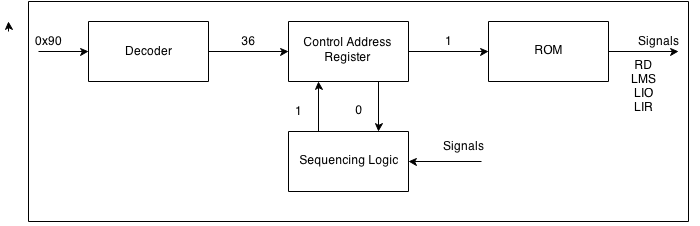
\includegraphics[scale=0.6]{FifthFlow}
    \end{center}
    \caption{Flow of instruction 2.(b)}
\end{figure}

\subsection{Coming Back to Fetch} \textbf{The states zero and one are maintained to be the fetch and decode micro-instruction cycles.} After RMS resets the sequencer state to zero, it again fetches the instruction in the next cycle by -

\begin{enumerate}
    \item At state zero, it will emit EPC LMR IPC to Load the Memory Address Register              with the value of the program counter.
    \item Then after state zero it will go to state one and emit RD LMS LIO LIR to load            the I/O Register, Instruction Register and the Micro Sequencer with the next
          instruction from the memory.
\end{enumerate}
Thus, the processor runs indefinitely till instructions are given.

\begin{figure}[h]
    \begin{center}
        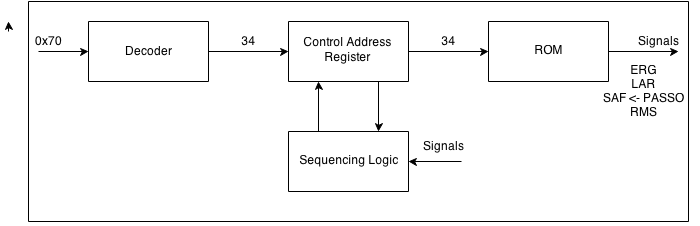
\includegraphics[scale=0.6]{ThirdFlow}
    \end{center}
    \caption{Flow of instruction 2.(c)}
\end{figure}

In the example the next instruction is \textit{movs r0}. Thus this instruction will cause the micro sequencer to change to the specific state with the micro-instruction. Thus the RMS of the prev instruction will cause state to be reset and the next instruction be fetched and executed.

\subsection{How and from Where the First Fetch ?} The initial state when the processor starts, is set to zero. Thus it fetches the instruction present at [[PC]] and executes it. Also, the PC is set to zero too and hence the first word from memory is fetched and executed on start up.